% Paper A draft (A8.2), started 10 Nov 2026. IEEE two-column conference format (fits TCAS-II brief after cuts, or FCCM).
% Every number is traced to a file in results/ (see paper/outline.md). \pend{...} marks items still to confirm.
% Revised 11 Nov 2026 after an external review (scope of the safety claim, full-width proof, resource accounting,
% heuristic comparison with charged reads, energy and real-time wording, architecture figure, reproducibility).
\documentclass[conference]{IEEEtran}
\usepackage{amsmath,amssymb,amsthm}
\usepackage{booktabs}
\usepackage{graphicx}
\usepackage{xcolor}
\usepackage{cite}
\usepackage{siunitx}
\usepackage{tikz}
\usetikzlibrary{arrows.meta,positioning,fit,calc}
\newcommand{\pend}[1]{\textcolor{red}{[#1]}}
\newtheorem{theorem}{Theorem}
\newtheorem{corollary}{Corollary}

\begin{document}

\title{HUSH: Provably Safe Sub-Block Hibernation for\\Real-Time Event-Driven SNN Inference on FPGAs}
\author{\IEEEauthorblockN{Anubhav Jha and Rajat Subhra Chakraborty \pend{spelling to confirm}}
\IEEEauthorblockA{Department of Electrical Engineering / Computer Science and Engineering, IIT Kharagpur, India \pend{affiliations to confirm}}}
\maketitle

\begin{abstract}
In a fully connected spiking layer, most of the time and energy goes into fetching the weights of every neuron for
every input spike, although few neurons fire. We present HUSH, an output-side skipping scheme that puts a sub-block
of eight neurons to sleep for a timestep only when a cheap integer envelope proves that none of them can reach the
threshold. At every timestep the gated layer therefore emits exactly the spikes that the ungated update from its
current state would emit; only the state of sleeping neurons evolves approximately. The envelope combines the exact
maximum membrane potential of the sub-block with a per-input proxy table and is computed while the previous timestep
is processed; its arithmetic is verified formally at the implementation's bit widths. Trained with the gate in the loop, a 578-256-10 integer network on N-MNIST
runs on a Xilinx Artix-7 XC7A100T at 100\,MHz entirely on chip, from raw sensor events to the class: at 95.74\,\%
accuracy it is 2.44$\times$ faster than the same hardware with the gate off (115\,\textmu s vs.\ 280\,\textmu s per
inference; 98.21\,\% accuracy) with 57\,\% less active energy per inference (18.4 vs.\ 42.5\,\textmu J,
estimated from gate-level switching activity), and at 96.54\,\% 1.75$\times$ faster with 44\,\% less. On the same chip and
weights as BASE, the open Spiker+ generator needs 818\,\textmu s and 255\,\textmu J (6.0$\times$ BASE). In cycle-accurate RTL replay of
N-MNIST event streams at their recorded timing, every 3\,ms window is processed within 4.5\,\textmu s of its end,
and the design sustains up to 1.33--2$\times$ the event rate of the ungated design with the same 1,024-event input
buffer.
\end{abstract}

\section{Introduction}
Event-driven spiking neural networks (SNNs) are attractive for always-on sensing because their input is sparse
and their arithmetic is additive. On FPGAs, accelerators usually exploit \emph{input} sparsity: work is done only
for input spikes that occur. For a fully connected layer with $N$ neurons, each input spike still costs $N$ weight
reads from block RAM, although in a given timestep only a few percent of the neurons fire. Skipping the
\emph{output} side, i.e.\ neurons that will not fire, is the remaining large saving, but it is hard: whether a
neuron fires depends on the very weights one wants to skip. Published output-side schemes are heuristics (they
predict that a neuron stays silent and can be wrong) and therefore change the network's behaviour in ways that are
hard to bound.

We make output-side skipping \emph{provably safe}. Our contributions:
\begin{enumerate}
\item \textbf{HUSH gate:} an integer envelope per sub-block of eight neurons that upper-bounds every member's next
membrane potential from the sub-block's exact current maximum and a per-input proxy table; a sub-block sleeps only
if the bound is below threshold (Theorem~1), so at every timestep the gated layer emits exactly the spikes of the
ungated update from its current state. We separate this per-timestep guarantee from end-to-end equivalence, which it
does not give, and measure the difference. The RTL arithmetic is proved safe for all values at its real bit widths.
\item \textbf{Architecture:} an envelope unit overlapped with the processing of the previous timestep, per-sub-block
weight-column RAM enables, a whole network on chip (hidden layer, output layer overlapped one timestep behind, and an
integer class decision), and a stream front-end that accepts raw DVS events.
\item \textbf{Evaluation on one chip:} bit- and cycle-exact RTL against a golden model; gate-level activity-based
power; the same RTL with the gate off as baseline (BASE); Spiker+~\cite{spikerplus} on the same device with BASE's weights;
three training seeds per point; and real-time operation on N-MNIST event streams replayed at sensor timing.
\end{enumerate}

\section{Background and related work}
\textbf{Integer LIF.} Each neuron keeps a 16-bit saturating potential $V$. Per timestep $t$,
$U = \mathrm{sat}(L(V) + \sum_{j\in A_t} w_{j})$ with leak $L(V)=V-(V\gg k)$, $k=4$, INT8 weights and $A_t$ the
active inputs; the sum is exact before the single saturation. It spikes, $s=[U\ge\theta]$ ($\theta=64$), and keeps
$V' = U-\theta s$ (soft reset).

\textbf{FPGA SNN accelerators on N-MNIST.} Table~\ref{tab:sota} lists the designs we found that report N-MNIST
results on an FPGA. They differ in network (convolutional, recurrent, fully connected), device and power method;
two report no latency.

\textbf{Output-side skipping.} Three recent designs skip work for neurons predicted not to fire:
Early~\cite{early} stops accumulation for neurons whose partial sum of the largest weights stays below a tuned
threshold; SITRA~\cite{sitra} scores each output of a spiking transformer with a weight-MSB dot product and skips the
weight fetches of outputs it predicts silent, overlapping detection with the previous token; PS4~\cite{ps4}
speculates whether each neuron fires within a time window and recomputes the window step by step when a speculation
fails. Early and SITRA accept mispredictions: Early reports a 0.54\,\% mean accuracy loss over its benchmarks and
SITRA 1--2\,\%; PS4 trades mispredictions for recomputation time instead. All three use tuned thresholds or
speculation and are evaluated with architecture simulators and ASIC synthesis (28 or 65\,nm), not on an FPGA. SPARSH~\cite{sparsh}
skips zero weights, zero spikes and refractory neurons; C-STEP~\cite{cstep} and the early-stop of~\cite{cheng2025}
end inference early in time. HUSH differs in that its prediction is a proven bound: a sleeping sub-block cannot
contain a neuron that would fire at that timestep, the bound carries membrane state across timesteps, and its
granularity matches a block-RAM column, so a skip removes whole memory reads on an FPGA.

\section{The HUSH gate}
Neurons are grouped into sub-blocks $c$ of $b=8$. Two tables are derived offline from the weights: the proxy
$P_{jc}=\max_{i\in c} W_{ji}$ and the mean $Q_{jc}=\lfloor \mathrm{mean}_{i\in c} W_{ji}\rfloor$. The hardware keeps
$R_c=\max_{i\in c} V_i$ exactly after every timestep. Before the weights of timestep $t$ are fetched, the envelope
unit accumulates $D_c=\sum_{j\in A_t} P_{jc}$ and evaluates
\begin{equation}
E_c=\mathrm{sat}\big(L(R_c)+\max(0,D_c)\big),\qquad g_c=[E_c\ge\theta].
\end{equation}
\begin{theorem}[Safety]
If $g_c=0$, every neuron $i$ in sub-block $c$ has $U_i<\theta$ in the ungated update from the same state.
\end{theorem}
\begin{proof}
$L$ is monotone, so $L(V_i)\le L(R_c)$; $W_{ji}\le P_{jc}$ gives $\sum_{j\in A_t}W_{ji}\le D_c\le\max(0,D_c)$; and
$\mathrm{sat}$ is monotone. Hence $U_i\le E_c<\theta$.
\end{proof}
A sleeping sub-block skips its weight reads. Its neurons are updated with a shared mean-field drive,
$U_i=\mathrm{sat}(L(V_i)+\sum_{j\in A_t}Q_{jc})\le E_c<\theta$, so they cannot spike either, and $R_c$ stays exact.

\textbf{What is guaranteed and what is not.} Two properties must be kept apart (Fig.~\ref{fig:scope}).
(A)~\emph{Per-timestep safety}: from HUSH's own state $V^{\mathrm H}_{t-1}$, the gated update emits exactly the
spikes of the ungated update, since awake sub-blocks are computed exactly and sleeping ones contain no neuron that
would reach $\theta$. This holds at every timestep, by Theorem~1. (B)~\emph{Trajectory equivalence} with an ungated
run, $V^{\mathrm H}_t=V^{\mathrm B}_t$, is \emph{not} guaranteed: a sleeping neuron receives the mean-field drive
instead of its own, so its state, and later spikes, can differ. We measured both on 1,000 test samples per point:
the golden model's shadow update finds no spike that HUSH suppresses relative to (A), while the hidden spike trains
of the same weights run with and without the gate diverge early (median first difference in window 4; 1.2--1.9\,\%
of spike bits differ) and end in the same class for 90--96\,\% of samples. Accuracy is therefore the measure of the
approximation in (B), and the gate is trained into the network for that reason.

\begin{figure}[t]\centering
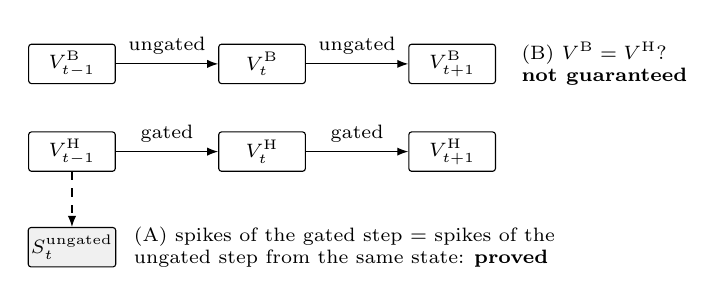
\begin{tikzpicture}[font=\scriptsize, st/.style={draw,rounded corners=1pt,minimum width=11mm,minimum height=5mm,inner sep=1pt},
  ar/.style={-{Latex[length=1.4mm]}}]
\node[st] (h0) {$V^{\mathrm H}_{t-1}$};
\node[st,right=13mm of h0] (h1) {$V^{\mathrm H}_{t}$};
\node[st,right=13mm of h1] (h2) {$V^{\mathrm H}_{t+1}$};
\draw[ar] (h0) -- node[above]{gated} (h1);
\draw[ar] (h1) -- node[above]{gated} (h2);
\node[st,below=7mm of h0,fill=black!6] (u1) {$S^{\mathrm{ungated}}_{t}$};
\draw[ar,dashed] (h0) -- (u1);
\node[right=1mm of u1,align=left] {(A) spikes of the gated step $=$ spikes of the\\ungated step from the same state: \textbf{proved}};
\node[st,above=6mm of h0] (b0) {$V^{\mathrm B}_{t-1}$};
\node[st,right=13mm of b0] (b1) {$V^{\mathrm B}_{t}$};
\node[st,right=13mm of b1] (b2) {$V^{\mathrm B}_{t+1}$};
\draw[ar] (b0) -- node[above]{ungated} (b1);
\draw[ar] (b1) -- node[above]{ungated} (b2);
\node[right=2mm of b2,align=left] {(B) $V^{\mathrm B}=V^{\mathrm H}$?\\\textbf{not guaranteed}};
\end{tikzpicture}
\caption{Scope of the guarantee. (A) holds at every timestep; (B) does not, because sleeping neurons receive the
mean-field drive. Measured on 1,000 samples: 0 spikes violate (A); trajectories differ from window 4 (median).}
\label{fig:scope}\end{figure} We train with the gate in the loop: the
forward pass uses the hard gate, and gradients flow through whichever update (exact or mean-field) it selected. Two
penalties are added to the cross-entropy: the envelope's mean excess over the
threshold, $\lambda_e\,\mathrm{mean}_{c,t}\max(0,E_c-\theta)/\theta$, and the expected positive proxy drive per
timestep, $\lambda_d\,\mathrm{mean}_c\sum_j r_j\max(0,P_{jc})/\theta$ with $r_j$ the firing rate of input $j$,
which shrinks the largest weight of each sub-block. The three points use $(\lambda_e,\lambda_d)=$ (0.25, 0.1)
gentler, (0.5, 0.25) gentle and (2, 1) aggressive; larger weights put more sub-blocks to sleep at some cost in
accuracy.

\section{Architecture}
\begin{figure*}[t]\centering
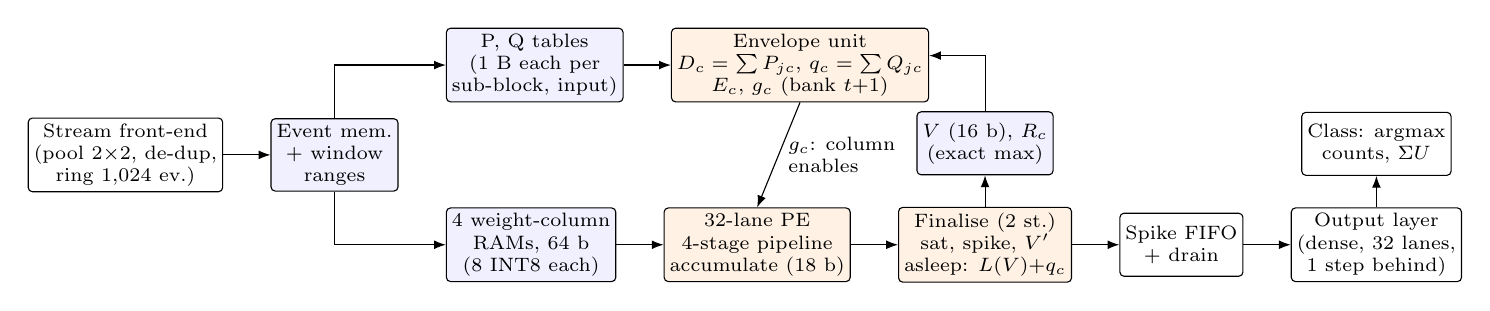
\begin{tikzpicture}[font=\scriptsize, bx/.style={draw,rounded corners=1.5pt,align=center,minimum height=8mm,inner sep=2pt},
  mem/.style={bx,fill=blue!6}, ctl/.style={bx,fill=orange!10}, ar/.style={-{Latex[length=1.5mm]}}]
\node[bx] (fe) {Stream front-end\\(pool 2$\times$2, de-dup,\\ring 1,024 ev.)};
\node[mem,right=6mm of fe] (ev) {Event mem.\\+ window\\ranges};
\node[mem,above right=2mm and 6mm of ev] (pq) {P, Q tables\\(1 B each per\\sub-block, input)};
\node[ctl,right=6mm of pq] (etu) {Envelope unit\\$D_c=\sum P_{jc}$, $q_c=\sum Q_{jc}$\\$E_c$, $g_c$ (bank $t{+}1$)};
\node[mem,below right=2mm and 6mm of ev] (w) {4 weight-column\\RAMs, 64 b\\(8 INT8 each)};
\node[ctl,right=6mm of w] (pe) {32-lane PE\\4-stage pipeline\\accumulate (18 b)};
\node[ctl,right=6mm of pe] (fin) {Finalise (2 st.)\\sat, spike, $V'$\\asleep: $L(V){+}q_c$};
\node[mem,above=4mm of fin] (vr) {$V$ (16 b), $R_c$\\(exact max)};
\node[bx,right=6mm of fin] (fifo) {Spike FIFO\\+ drain};
\node[bx,right=6mm of fifo] (l2) {Output layer\\(dense, 32 lanes,\\1 step behind)};
\node[bx,above=4mm of l2] (cls) {Class: argmax\\counts, $\Sigma U$};
\draw[ar] (fe) -- (ev);
\draw[ar] (ev) |- (pq);
\draw[ar] (ev) |- (w);
\draw[ar] (pq) -- (etu);
\draw[ar] (etu.south) -- node[right,align=left]{$g_c$: column\\enables} (pe.north);
\draw[ar] (w) -- (pe);
\draw[ar] (pe) -- (fin);
\draw[ar] (fin) -- (vr);
\draw[ar] (vr.north) |- ($(etu.east)+(0,0.12)$);
\draw[ar] (fin) -- (fifo);
\draw[ar] (fifo) -- (l2);
\draw[ar] (l2) -- (cls);
\end{tikzpicture}
\caption{HUSH whole-network datapath. The envelope unit computes the gates of timestep $t{+}1$ from the proxy and mean
tables while the PE processes timestep $t$; a sub-block's weight column is read only when its gate is set. Blue:
memories; orange: HUSH-specific logic and the lanes it controls.}\label{fig:arch}\end{figure*}

\textbf{Hidden layer.} 256 neurons form 8 blocks of 32 lanes (4 sub-blocks of 8). The weight memory is four 64-bit
column RAMs, one per sub-block; a column is read only if its sub-block is awake. Per timestep the sequencer combines
the envelope bank (gates), then visits each block: an awake block streams the timestep's events through a
4-stage pipeline (event read, index register, weight read, accumulate) and finalises its lanes in two stages; an
asleep block takes 3 cycles (state read, mean-field finalise, write-back). The envelope unit for timestep $t+1$
runs during the block loop of $t$ (double-buffered banks). The cycle cost of a timestep with $n>0$ events is
$1 + \sum_b c_b + 2$ with $c_b = 4 + (n+4)$ for an awake block and 3 for an asleep one, plus any wait for the
envelope bank. Time is therefore saved per 32-neuron block (all four sub-blocks asleep), while energy is also saved per
8-neuron sub-block, whose weight column is not read.

\textbf{Whole network.} Hidden-layer spikes enter a 32-entry FIFO; a drain converts each set bit into an event of the
output layer (32 lanes, 10 used, dense), which runs one timestep behind the hidden layer and overlapped with it.
The class is the integer argmax of spike counts, ties broken by the summed pre-reset potential, then by index.

\textbf{Stream front-end.} Raw DVS events $(x,y,p)$ are pooled $2\times2$ into the 578 inputs, de-duplicated per
window (the model's input is a 0/1 raster), and written into a ring of 1,024 events (one RAMB18); an end-of-window
marker closes the window, writes its range and lets the hidden layer start its envelope pass for that window.
Markers have reserved FIFO space, so overload can only drop events. In stream mode the whole network takes
8,736 LUTs / 48.5 BRAMs (BASE) and 14,606 / 62.5 (HUSH), both at 100\,MHz.

\section{Verification}
A golden integer model (Python) defines the behaviour. The RTL matches it bit for bit on 80 randomised layer
configurations (gate, mean-field, sizes, leak, threshold, load port) and, for the whole network, on 50 N-MNIST test
samples for each of four weight sets: every hidden and output block result and every class, with cycle counts equal
to an exact cycle model. Forty random whole networks (including a 4-entry spike FIFO that forces back-pressure) are also bit-exact. The
stream mode is bit-exact in every run without dropped events, at true sensor timing and up to 2,000$\times$ replay. The
safety arithmetic is verified formally with SymbiYosys (ABC PDR) on the RTL modules used in the design, in two
complementary checks. (1)~At the implementation's widths (16-bit $V$, 18-bit accumulators, $k=4$, $\theta=64$; both
the 578-input and the 256-input layer), one timestep of an 8-lane sub-block with every value free proves that, if
each $V_i\le R_c$ and each neuron's drive is at most $D_c$: a sleeping sub-block contains no neuron whose ungated $U$
reaches $\theta$; every $U_i\le E_c$, awake or asleep; no sum wraps around (each 18-bit result equals the same sum
computed 8 bits wider); and $R'=\max V'$ restores the hypothesis. With $V=R=0$ at reset this is an induction over
timesteps (72\,s). (2)~A sequential model at reduced widths proves the same properties over unbounded time for both
sleep semantics. Mutants with an unsafe proxy fail both checks immediately. Table~\ref{tab:widths} lists the bounds;
the proxy and mean tables are generated offline and checked by the bit-exact simulations, which also cover memories
and sequencing.

\begin{table}[t]\centering\caption{Widths and the values that can occur (hidden layer, $M=578$).}\label{tab:widths}
\setlength{\tabcolsep}{3pt}\footnotesize
\begin{tabular}{lll}\toprule
Quantity & Width & Range that can occur\\\midrule
$W$, $P$, $Q$ & 8 b & $[-128,127]$\\
$V$, $R$ ($L(V)$) & 16 b & $[-32768,32767]$ ($|L(V)|\le 30720$)\\
$D_c$, $q_c$ ($\le 578$ inputs) & 18 b & $[-73984,73406]$\\
Lane sum $L(V)+\sum W$ & 18 b & $[-104704,104126]$ (18 b: $\pm131072$)\\
$U$, $E$ after the clip & 16 b & saturated\\
Class $\Sigma U$ per output & 32 b & $|\Sigma U|\le 3.28\,$M\\\bottomrule
\end{tabular}\end{table} Gate-level simulation of the routed
netlists reproduces the model's cycle count for every inference (+3 cycles of restart).

\section{Results}
\textbf{Setup.} XC7A100T-1CSG324C, Vivado 2024.1, 100\,MHz. Power is Vivado's estimate (\texttt{report\_power})
annotated with the gate-level switching activity (SAIF) of 20 back-to-back test inferences on the routed netlist
(99.9--100\,\% of nets matched, confidence High); it is not a board measurement. Energy per inference $=$ power
$\times$ latency while the chip is processing (\emph{active} energy; Section~VII discusses energy at sensor speed).
Accuracy on the full 10,000-sample N-MNIST test set ($T=100$ windows of 3\,ms) with the hardware's integer decision
rule; accuracy and latency over three training seeds; area, power and energy for the seed-0 networks on 20 samples.
BASE's power and energy were estimated with its own (22-epoch) weights; they equal those of the 10-epoch BASE
(152\,mW, 42.5\,\textmu J). Training (Table~\ref{tab:train}) uses the integer model of Section~II in PyTorch and
keeps the final epoch (no model selection on the test set).

\begin{table}[t]\centering\caption{Training setup (all points, N-MNIST).}\label{tab:train}
\setlength{\tabcolsep}{3pt}\footnotesize
\begin{tabular}{@{}lp{0.74\columnwidth}@{}}\toprule
Input & 34$\times$34$\times$2 events, 2$\times$2 pooling $\rightarrow$ 578; $T=100$ windows of 3\,ms; 0/1 raster\\
Network & 578-256-10 integer LIF, $k=4$, $\theta=64$, soft reset, 16-bit $V$\\
Weights & INT8: round-and-clamp in the forward pass, straight-through gradient\\
Spike gradient & fast sigmoid, $1/(s(1+|x|/s))^2$ with $s=\theta/4$\\
Readout loss & cross-entropy on $(\#\text{spikes}+0.01\,\overline{U}/\theta)\cdot 25/T$\\
Regulariser & $5\cdot\max(0,\bar r-0.05)$ on the hidden firing rate $\bar r$\\
Optimiser & Adam, one-cycle schedule (15\,\% warm-up), batch 128\\
BASE & 10 epochs, peak lr 0.05; then 12 epochs from it, lr 0.02 (no gate)\\
HUSH & 12 epochs from 10-epoch BASE, lr 0.02, gate in the loop, $\lambda_e,\lambda_d$ per point\\
Seeds & 0, 1, 2 (weight init and batch order)\\\bottomrule
\end{tabular}\end{table}

\begin{table}[t]\centering\caption{Accuracy and latency, whole network on chip (mean $\pm$ std, 3 seeds; latency over 500 test samples).}\label{tab:front}
\setlength{\tabcolsep}{2.5pt}\small
\begin{tabular}{lcccc}\toprule
Design & Acc.\ (\%) & Reads$^c$ & Lat.\ (\textmu s) & Speedup$^e$\\\midrule
BASE (gate off)$^b$ & 98.21$\pm$0.13 & 1.000 & 279.5 & 1.00$\times$\\
HUSH gentler & 96.54$\pm$0.07 & 0.204 & 159.8$\pm$8.1 & 1.75$\times$\\
HUSH gentle & 95.74$\pm$0.07 & 0.118 & 114.9$\pm$7.0 & 2.44$\times$\\
HUSH aggressive & 92.32$\pm$0.68 & 0.070 & 82.9$\pm$7.8 & 3.39$\times$\\\bottomrule
\multicolumn{5}{p{0.95\columnwidth}}{\footnotesize $^b$ trained as long as the gated nets (10 + 12 epochs); 10 epochs only: 97.66$\pm$0.07. $^c$ weight-column reads relative to BASE; adding HUSH's own reads of $P$ and $Q$ (2\,B per sub-block and input,
vs.\ 8\,B per column), its total weight-memory traffic is 0.32--0.45 of BASE's. $^e$ mean of the per-seed ratios.}
\end{tabular}\end{table}

\begin{table}[t]\centering\caption{Hardware on XC7A100T, 100\,MHz (whole network, 20 on-chip samples).}\label{tab:hw}
\setlength{\tabcolsep}{2.5pt}\small
\begin{tabular}{lccccccc}\toprule
Design & LUT & BRAM & WNS & Lat. & Power & Energy \\
 & & & (ns) & (\textmu s) & (mW) & (\textmu J)\\\midrule
BASE & 7,745 & 80 & +0.956 & 279.5 & 152 & 42.5\\
HUSH gentler & 13,885 & 95 & +0.450 & 151.2 & 157 & 23.7\\
HUSH gentle & 13,885 & 95 & +0.450 & 115.3 & 160 & 18.4\\
HUSH aggr. & 13,885 & 95 & +0.450 & 87.7 & 164 & 14.4\\
Spiker+~\cite{spikerplus} & 13,548$^a$ & 70.5 & +0.005$^a$ & 818.4 & 311 & 254.5\\\bottomrule
\multicolumn{7}{p{0.95\columnwidth}}{\footnotesize Latency and power over the 20 simulated inferences; static power 101--102\,mW.}\\
\multicolumn{7}{p{0.95\columnwidth}}{\footnotesize $^a$ high-effort implementation; power measured on the default-effort netlist (WNS $-$0.241\,ns).}
\end{tabular}\end{table}

\textbf{Accuracy--savings front.} Table~\ref{tab:front}. The gated networks are fine-tuned for 12 epochs from the
10-epoch ungated network; the same fine-tuning without the gate raises the ungated network from 97.66\,\% to
98.21\,\%, so we use that network as BASE. Against it the gate costs 1.7--5.9 points and reads 7--20\,\% of the
weight columns. Training longer with the gate (12 instead of 6 epochs) improved every
axis of the gentle point (95.37\,\%, 1.98$\times$ $\rightarrow$ 95.74\,\%, 2.44$\times$). In a single-seed test, a wider hidden layer (384) raised the ungated accuracy to 98.0\,\% but not the gated one
(95.9\,\%, 6 epochs).

\textbf{Same chip.} Table~\ref{tab:hw} gives the power builds; Table~\ref{tab:res} reconciles them with the stream
builds. A power build stores 20 test recordings on chip (53k events, $\approx$32.5 BRAM tiles) so that power can be
simulated over 20 inferences without a host; a stream build instead has the sensor front-end and a 1,024-event
ring. HUSH adds the same $\approx$6k LUTs and 14--15 BRAM tiles in both (envelope unit, $P$ and $Q$ tables,
sub-block control).

\begin{table}[t]\centering\caption{Resources of the four builds (BRAM in 36\,Kb tiles).}\label{tab:res}
\setlength{\tabcolsep}{2.2pt}\footnotesize
\begin{tabular}{lcccccc}\toprule
Build & \multicolumn{2}{c}{Hidden layer} & Output & Glue$^f$ & \multicolumn{2}{c}{Total}\\
 & LUT & BRAM & LUT/BRAM & LUT & LUT & BRAM\\\midrule
BASE, power & 3,874 & 74 & 3,117/6 & 754 & 7,745 & 80\\
HUSH, power & 9,922 & 89 & 3,150/6 & 813 & 13,885 & 95\\
BASE, stream & 4,482 & 41.5 & 3,142/7 & 1,112 & 8,736 & 48.5\\
HUSH, stream & 10,365 & 56.5 & 3,122/6 & 1,119 & 14,606 & 62.5\\\bottomrule
\multicolumn{7}{p{0.95\columnwidth}}{\footnotesize Power builds hold 20 recordings on chip (Table~\ref{tab:hw});
stream builds hold a 1,024-event ring and the sensor front-end (Section~IV). $^f$ spike FIFO, drain, classifier,
front-end and board harness (UART loader, LED fold); total minus the two layers. All four meet 100\,MHz (WNS +0.252 to +0.956\,ns).}
\end{tabular}\end{table} Spiker+ (clock-driven, ungated) runs BASE's 10-epoch INT8 weights (97.53\,\% on its neuron semantics, fixed point
with 6 fractional bits), scans all 578 inputs serially each timestep and needs 81.8k cycles per inference in our
harness (81.4k for the bare generated network). With default implementation settings it misses 100\,MHz by
0.24\,ns; with high-effort directives it meets 100\,MHz (+0.005\,ns, 13,548 LUTs). Its power was measured on the
default-effort netlist; the high-effort one is estimated 4\,\% higher, so the reported Spiker+ energy is a lower
bound. With the gate, HUSH spends 44--66\,\% less energy
per inference than BASE although its power is 3--8\,\% higher: the extra envelope logic costs less than the time it
saves; this is active energy per inference. Spiker+ draws 311\,mW, 140\,mW of it in block RAM, which it reads every cycle (ours: 12\,mW, read only for
awake sub-blocks), and needs 6.0$\times$ the energy of BASE and 13.8$\times$ that of HUSH gentle. Energies in
Table~\ref{tab:hw} use the latency of the same 20 inferences (e.g.\ gentler 151.2\,\textmu s vs.\ 159.8\,\textmu s over
500 samples); the speedups of Table~\ref{tab:front} use the 500-sample means.

\textbf{Heuristic gates.} On the 6-epoch gentle network and 200 test samples, we replaced only the predictor and
bisected each heuristic's threshold to HUSH's read fraction (0.157): a state-free proxy inspired by SITRA (count of
negative weights of the active inputs; not SITRA's MSB dot product) reaches 66.0\,\% and suppresses 15,121 spikes; an
Early-style predictor ($L(V)$ plus the top-8 active weights) 93.5\,\% with 36; HUSH 95.5\,\% with none. Two caveats
favour HUSH: the network was trained with the HUSH gate, not with the heuristics, and the Early-style predictor's own
weight reads are not charged.

\section{Real-time operation}
N-MNIST recordings deliver on average 41.9 raw events per 3\,ms window (26.5 distinct pooled inputs; maximum 96).
Real-time feasibility is shown by cycle-accurate RTL replay of N-MNIST event streams at their recorded timing,
not by a sensor connected to the board. \textbf{At true sensor timing} (4 recordings per design, bit-exact, no drops) a window is processed in
1.47\,\textmu s on average with HUSH (3.04\,\textmu s BASE), at most 4.50\,\textmu s (6.64\,\textmu s), i.e.\
$\le 0.22$\,\% of the window; the class is ready 0.89\,\textmu s (2.03\,\textmu s) after the last window; the input
ring never holds more than 127 events. HUSH shortens the average window (by 37\,\%), not the busiest one, where
most blocks wake up (840 vs.\ 828 cycles).
\textbf{Energy in real-time operation.} The 44--66\,\% saving of Section~VI is active energy per inference. At sensor
speed the chip idles more than 99.9\,\% of the time, so a 300\,ms recording costs $\approx$30.3\,mJ of static energy
(101\,mW) for either design, and HUSH saves only its dynamic share (6.7 vs.\ 14.3\,\textmu J per inference), i.e.\
$<0.03$\,\% of the always-on total. HUSH's gain appears when the chip is kept busy, e.g.\ serving recordings
faster than real time: at the highest replay speed that drops nothing on the heaviest recordings (750$\times$ BASE,
1,000$\times$ HUSH gentle) a recording costs 152\,mW$\times$0.40\,ms $=$ 61\,\textmu J with BASE and
160\,mW$\times$0.30\,ms $=$ 48\,\textmu J with HUSH.
\textbf{Faster than real time.} Replaying the 20 test recordings with the most events (1.7$\times$ the mean rate)
with the same 1,024-event buffer, BASE drops events above 750$\times$ real time, HUSH gentle above 1,000$\times$ on
all 20 recordings (23.7\,M events/s, 1.33$\times$) and above 1,500$\times$ for the median recording (2.0$\times$).
\textbf{Early decisions.} Because the class can be read after any window, Fig.~\ref{fig:early} reports accuracy vs.
elapsed sensor time. Between 21\,ms and 156\,ms the gentler network is more accurate than BASE trained equally long
(e.g.\ 87.7\,\% vs.\ 79.5\,\% at 60\,ms and 92.6\,\% vs.\ 88.9\,\% at 99\,ms); BASE leads from 159\,ms on.
The gated networks do not spike earlier or more (fewer output spikes in the first 99\,ms: 39--41 vs.\ 52) but
their early leading class is wrong less often (8.5--8.8\,\% vs.\ 10.6\,\% of 1,000 samples at 99\,ms).
The gentle network leads from 21\,ms to 144\,ms. An application that must decide within $\approx$140\,ms is
therefore both faster and more accurate with either gated network. (Spike statistics: first 1,000 test samples.)
\begin{figure}[t]\centering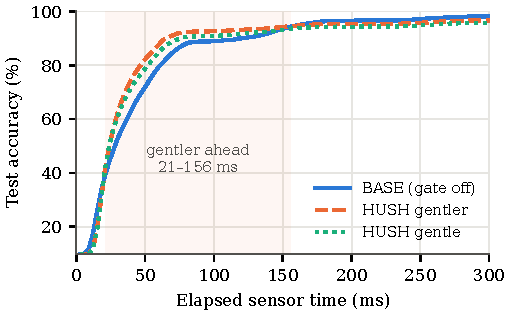
\includegraphics[width=\columnwidth]{fig_early.pdf}\caption{Accuracy when the class is read after the first windows of a recording (10,000 test samples). BASE is trained as long as the gated networks.}\label{fig:early}\end{figure}

\section{Comparison with the state of the art}
\begin{table}[t]\centering\caption{FPGA SNN accelerators on N-MNIST.}\label{tab:sota}
\setlength{\tabcolsep}{2pt}\footnotesize
\begin{tabular}{lccccc}\toprule
Design & FPGA & Acc.\ (\%) & LUT & Power & Latency\\\midrule
Cheng et al.~\cite{cheng2025} & ZCU104 & 98.11 & 81.3k & 0.81$^d$ & n/r\\
FeNN-DMA~\cite{fenndma} & KV260 & 98.46 & 55.0k & 0.53$^d$ & n/r\\
Surrogates~\cite{surr2026} & xcvu9p & 96.4 & n/r & 0.31 & 5.9\,ms\\
Wu et al.~\cite{wu2023} & ZCU102 & 95.76 & 39.7--165k & 0.33--0.37 & 50\,ms\\
\textbf{HUSH gentler} & XC7A100T & 96.54 & 13.9k & 0.16/0.056$^d$ & 0.16\,ms\\
\textbf{HUSH gentle} & XC7A100T & 95.74 & 13.9k & 0.16/0.058$^d$ & 0.11\,ms\\\bottomrule
\multicolumn{6}{l}{Power in W; $^d$ dynamic only; n/r: not reported.}
\end{tabular}\end{table}
HUSH runs 37--435$\times$ faster per inference than the designs that report latency and needs 77--950$\times$ less
active energy per inference (18.4--23.7\,\textmu J vs.\ $\approx$1.83 and $\approx$17.5\,mJ computed by us as their power
$\times$ latency), on a smaller device with
4--6$\times$ fewer LUTs than the two designs that report them (3--12$\times$ fewer than Wu et al.'s range). Accuracy
is comparable to those two designs (96.54 vs.\ 96.4 and 95.76\,\%) and 1.6--1.9 points below the two larger designs;
with the gate off, the same hardware reaches 98.21\,\% at 280\,\textmu s. These rows are not like for like.
\emph{Networks}: Cheng et al.\ and Wu et al.\ use fully connected event-driven SNNs, FeNN-DMA a 512-neuron recurrent
network, the Surrogates design a VGG9-style convolutional SNN; ours is 578-256-10. \emph{Devices}: all others use
UltraScale+ parts with 1.8--19$\times$ the LUT capacity of the XC7A100T. \emph{Latency}: ours is the compute time of one 300\,ms recording
whose events are already on chip; the others report their own per-sample processing time. \emph{Power}: ours and
Cheng et al.'s are Vivado estimates from simulated activity, FeNN-DMA's is a vectorless estimate with the processing
system removed; the Surrogates and Wu et al.\ figures are as reported, and their energies are computed by us. Only the same-chip comparison
(Tables~\ref{tab:front}--\ref{tab:res}) isolates HUSH's own effect.

\section{Limitations and conclusion}
The speedup depends on stream sparsity: per window it falls from 2.2$\times$ with fewer than 10 active inputs to
1.6$\times$ with more than 60, as more sub-blocks wake up, and it tends to 1$\times$ on dense streams. Serving many
streams on one chip is limited by state memory, where BASE would fit more streams than HUSH. The gate costs accuracy;
its guarantee is per timestep, not for the whole trajectory; power is estimated from simulated activity, not measured
on a board; and real time is shown by RTL replay at sensor timing, not with a live sensor. HUSH shows that output-side skipping in SNN hardware can be both effective and provably safe; extending
the envelope to convolutional layers and denser event streams (DVS-Gesture) is future work.

\bibliographystyle{IEEEtran}
\bibliography{refs}
\end{document}
